\chapter{Tangibilidade é decidível}

\section{Lema do princípio da casa dos pombos}

\figuradoautor{Princípio da casa dos pombos}{
    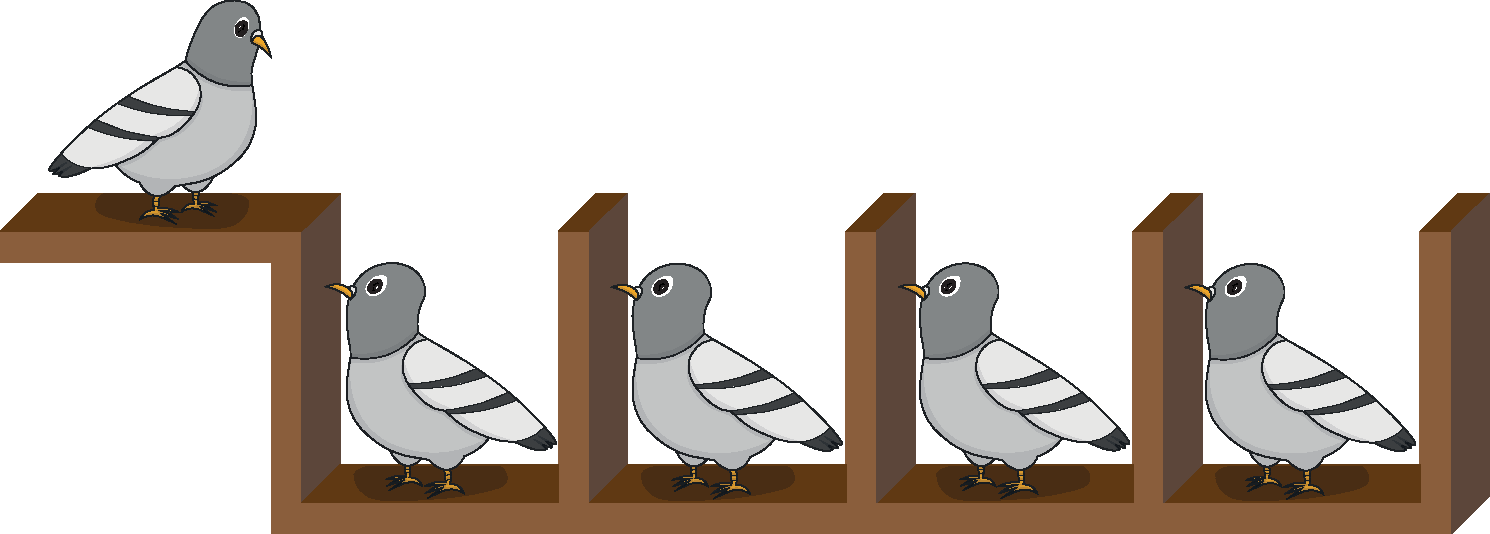
\includegraphics[width=.8 \textwidth]{imagens/pombos.pdf}
}{fig:afd_diagrama}

\begin{minted}{coq}
Lemma casa_dos_pombos : forall (l1 l2:A),
  (forall x, In x l1 -> In x l2) ->
  length l1 > length l2 ->
  repete l2.
\end{minted}

De acordo com \citeonline{jesper} e \citeonline{pierce}, a prova do lema \mintinline{coq}{casa_dos_pombos} não exige \begin{equation}\label{eq:InA_dec}\text{\mintinline{coq}{forall (a:A) l, {In a l} + {~ In a l}}}\end{equation} mas a demonstração de outra forma torna-se muito mais extensa. Para os propósitos deste trabalho, não obstante, o Coq tem, em sua biblioteca padrão, uma prova para a Equação \ref{eq:InA_dec} -- \mintinline{coq}{in_dec} -- sob a hipótese de que a igualdade de \mintinline{coq}{A} é decidível. Como a definição de AFD do presente trabalho restringe tal decidibilidade, a demonstração pode ser feita de modo trivial.

\begin{minted}{coq}
forall X:Type,
(forall (x y:X), {x = y} + {x <> y}) ->
forall (x:X) (l:list X), {In x l} + {~ In x l}
\end{minted}

\section{Lema do bombeamento}



\section{Computabilidade e decidibilidade do problema}

Ao avaliar a computabilidade de um problema, as complexidades de tempo e espaço não são fatores limitantes.
